% #############################################################################
% This is Chapter 4
% !TEX root = ../main.tex
% #############################################################################
% Change the Name of the Chapter i the following line
\fancychapter{Implementation}
\cleardoublepage
% The following line allows to ref this chapter
\label{chap:implementation}

\par In this chapter, implementation in both Matlab and Python will be discussed. This chapter focuses on formalising the optimisation problem for multipe vehicles. Once the optimisation problem is formalised, it can be solved by a whole range of non linear optimisation algorithms.

\par The Motion Planning problem for multiple vehicles that will be focused for the project consists in a go-to formation manoeuvre \cite{sabetghadam2018cooperative}. The go-to formation manoeuvre consists of the simultaneous arrival of a formation of vehicles to desired locations whilst simultaneously avoiding collisions between each other and the environment.

\par Just as for the case of optimisation for a single vehicle, motion planning for multiple vehicles will also be based on the minimisation of an appropriate cost function. This time, however, the cost will be the result of the sum of the costs of each individual vehicle and an added constraint will be necessary that will take into account inter vehicle collisions. 

\par The optimal control problem can be redefined for multiple vehicles as 
\begin{equation}
    \label{eq:multi_cost}
    \begin{aligned}
    & \underset{x^{[i]}(.),u^{[i]}(.),i= 1,\dots N_v}{\text{minimize}} && \int_0^T \sum_{i=1}^{N_v}  L_i (x^{[i]}(t),u^{[i]}(t))dt + \Psi (x(T)) \\
    & \text{subject to}  && x^{[i]}(0) = x_0^{[i]}, \\
        & && x^{[i]}(T) = x_f^{[i]}, \\
        & && \dot{x}^{[i]} = f_i (x^{[i]}(t), u^{[i]}(t)), &&& t \in [0,T]\\
        & && c_{col} (x^{[i]},u^{[i]} ) \geq 0, \\
        & && h(x(t),u(t)) \geq 0, \\
        & && \underline{x}^{[i]} \leq x^{[i]} (t) \leq \overline{x}^{[i]} , \\
        & && \underline{u}^{[i]} \leq u^{[i]} (t) \leq \overline{u}^{[i]}
    \end{aligned}
\end{equation}

\par This problem will also produce a solution within time horizon $T$. Initial and terminal constraints will exist for every vehicle, as well as inter-vehicle constraints.

\par A problem that only has the integral term $\sum_{v=1}^{N_v} L_v(x^{(v)}(t),u^{(v)}(t))$ is said to be in \textit{Lagrange form}, a problem that optimises only the boundary objective $\sum_{v=1}^{N_v} \Psi_v(x(T))$ is said to be in \textit{Mayer form} and a problem with both terms is said to be in \textit{Bolza form}. An example where only the \text{Mayer form} would be necessary could be a situation where the desired destination of the vehicles does not have enough room for them all to be arranged in their desired positions. Therefore, the goal of the optimiser is to find the closest to the desired positions.


\par There are 2 ways of preventing inter-vehicle collision; \textit{spatial deconfliction} and \textit{temporal deconfliction} \cite{hausler2015mission}.
Spatial deconfliction imposes the constraint that the spatial paths of the vehicles under consideration will never intersect and keep a desired safe distance from each other. Temporal deconfliction requires that two vehicles will never be ”at the same place at the same time”. However, their spatial paths are allowed to intersect. Figure \ref{fig:deconfliction} illustrates the two types of deconfliction strategies. Temporal deconfliction allows an extra degree of freedom and will intuitively lead to cheaper dynamic costs.

\par A simple method to assure temporal deconfliction of 2 vehicles is to assure that the norm of the distance of each point in time $t\in [0,T]$ is on each point in time subtract the n-dimensional trajectories of each pair of vehicle 

\begin{figure}
    \centering
    \begin{subfigure}[b]{0.45\textwidth}
        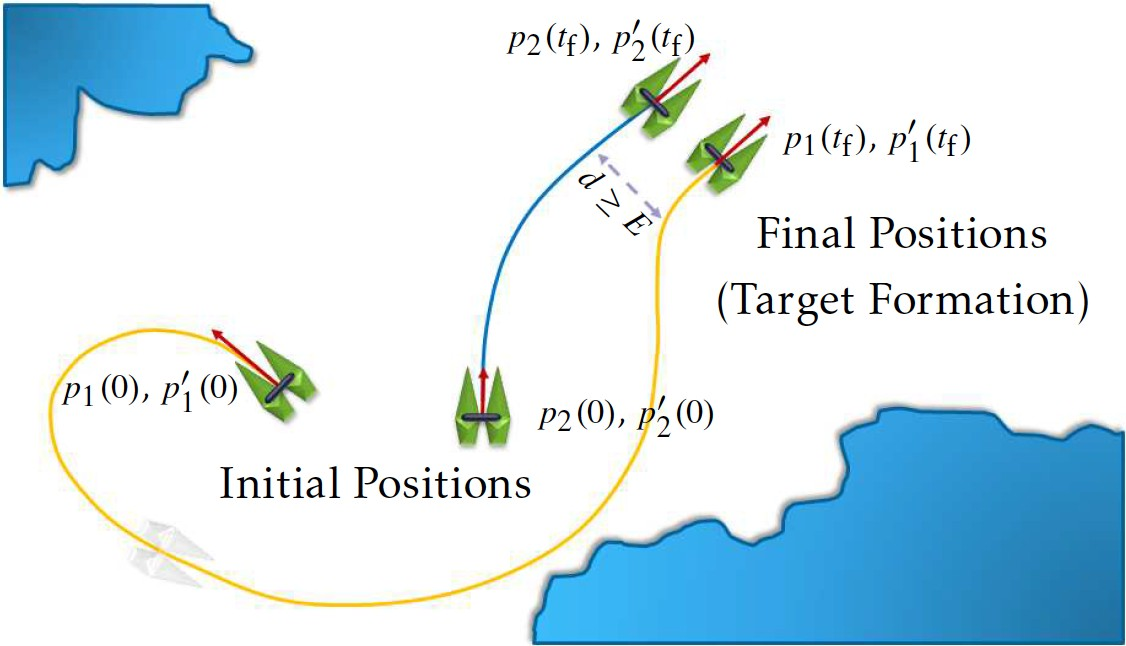
\includegraphics[width=\textwidth]{Images/spacial_deconf.jpg}
        \caption{Spacial Deconfliction}
    \end{subfigure}
    ~
    \begin{subfigure}[b]{0.45\textwidth}
        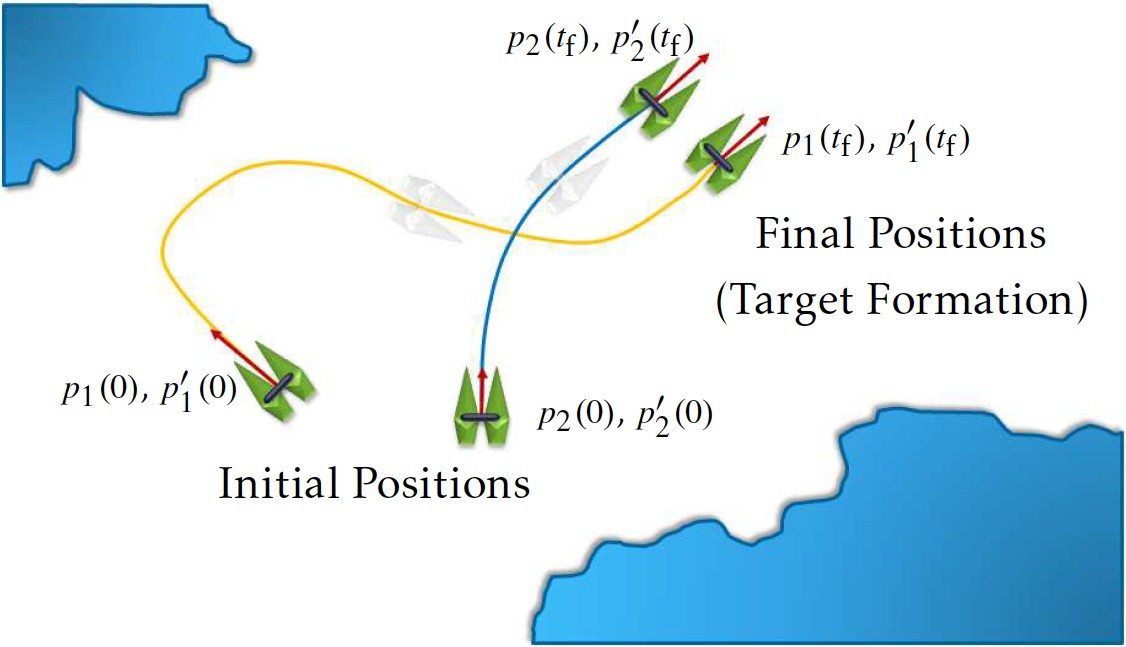
\includegraphics[width=\textwidth]{Images/temporal_deconf.jpg}
        \caption{Temporal Deconfliction}
    \end{subfigure}
    \caption{Inter Vehicle deconfliction Solutions}
    \label{fig:deconfliction}
\end{figure}

\section{Description of the implemented code}

\par The variables for the motion planning problem are each vehicle's state variables and inputs, as explained in chapter \label{chap:autonomousvehiclemodels}. Each of these variables will be refered to as curves. Optimisation algorithms cannot take continuous functions as variables, therefor, some form of parameterisation of each curve is necessary, as exemplified in some of the algorithms of chapter \label{chap:theory}. Here, each curve will be represetend as a Bernstein Polynomial with order $N$, which will require $N+1$ control points. A destinction is made between state variables and inputs: state variables must have establised initial and final conditions, inputs do not. This implies that for state variables, the initial and final control points must be fixed, therefor, they do not need to participate on the optimisation problem. The following matrix represents how the control points are stored so that they can be accessed by all functions that perfom operations on the curves

\begin{equation}
    \begin{bmatrix}
        \colorbox{yellow}{$\displaystyle x_0^0$} & \colorbox{yellow}{$\displaystyle y_0^0$} & \colorbox{yellow}{$\displaystyle \psi_0^0$} & \colorbox{yellow}{$\displaystyle u_0^0$} & \colorbox{yellow}{$\displaystyle v_0^0$} & \colorbox{yellow}{$\displaystyle r_0^0$} & \tau_{u_0}^0 & \tau_{r_0}^0 \\
        x_1^0 & y_1^0 & \psi_1^0 & u_1^0 & v_1^0 & r_1^0 & \tau_{u_1}^0 & \tau_{r_1}^0 \\
        \vdots & \vdots & \vdots & \vdots & \vdots & \vdots & \vdots & \vdots \\
        \colorbox{yellow}{$x_{N}^0$} & \colorbox{yellow}{$y_{N}^0$} & \colorbox{yellow}{$\psi_{N}^0$} & \colorbox{yellow}{$u_{N}^0$} & \colorbox{yellow}{$v_{N}^0$} & \colorbox{yellow}{$r_{N}^0$} & \tau_{u_{N}}^0 & \tau_{r_{N}}^0
    \end{bmatrix}
    \label{eq:matrixofvariables}
\end{equation}

\par It is believed \todo{can this be said? because I'm not referencing anything (I'm taking Venanzio's word for it)} that \texttt{fmincon()} performs better when all variables are stored in a line vector, therefor, a function called \texttt{matrify()} is necessary in order to transform the flattened optimisation variable to the matrix of equation (\ref{eq:matrixofvariables}). 
\par Elements marked in yellow do not participate in the optimisation algorithm. They are concatenated to this matrix in \texttt{matrify()}. 

\par High orders are preferable for each curve because \todo{reference "the paper" (of Venanzion, Isaac, Pascoal, etc) } the higher the curve, the closer the control points are to the "matching" point in time of the curve, which is achieved once an optimisation problem finishes. Chapter \ref{chap:results} exemplifies show the control points approximate to the curve and how it is advantageous to produce the dynamics.

\par A more precise way to calculate the minimum distance of a Bezier curve to a point or to another curve, compared to the one implemented on section \ref{sec:2_d_bezier} is via the algorithm presented in \cite{chang2011computation}. This algorithm takes into account the convex hull property of Bezier Curves and the \textit{deCasteljau} algorithm for subdividing curves. It will also employ the GJK algorithm, a fast and efficient way of calculating distances between 2 convex shapes\cite{cichella2018bernstein}.
\par The fast calculation of distances between these curves allows Bezeir Curves to be appropriate for testing non-linear constraints in multiple vehicle motion planning optimisation.

\par This fancy algorithm performed poorly because it was iterative. A simpler way to calculate the minimum distance was necessary. This consited in subtracting each pair of 2-D curves for each vehicle to eachother, then getting a rough guess of the closest point of that resulting curve to 0: by performing degree elevation to an order 10 times the original then looking for the closest point to the origin. 

\par Minimum distance of the curves to objects was done with GJK. but it was slow

\par Collision to circles is calculated by subtracting the 2-D curve tto the centre of the circle, performing degree elevation of the resultign curve, calculating the closest to the origin and checking wether that distance is greater to the radius. Performing the check for every control point was also done but wasn't advantageous (slower runtime), the reason could be because the derivative of each of these distances or the elevated curve with respect to the position of the control points depends on more than 1 control points of the non elevated curve, therefor, some computation is redundant.


\par The optimisation problem is formulated by constructing a data structure with the fields of table \ref{tab:constants_description}. In Python the same fields are necessary, however, they must be stored in a python dictonary. 


\begin{table}[]
\centering
\begin{tabular}{|l|l|l|l|}
\hline
\textbf{field} & \textbf{description} & \textbf{mandatory} & \textbf{example} \\ \hline
\texttt{T} & Time horizon & yes & \texttt{10} \\ \hline
\texttt{xi} & initial conditions & yes & \texttt{[0 0 0 1 0]} \\ \hline
\texttt{xf} & final conditions & yes & \texttt{[5 5 pi/2 1 0]} \\ \hline
\texttt{N} & order of the curves & yes & \texttt{15} \\ \hline
\texttt{obstacles} & polygons & \begin{tabular}[c]{@{}l@{}}no\\ default: \texttt{[]}\end{tabular} &  \\ \hline
\texttt{obstacles\_circles} & circles & \begin{tabular}[c]{@{}l@{}}no\\ default: \texttt{[]}\end{tabular} &  \\ \hline
\texttt{min\_dist\_int\_veh} & \begin{tabular}[c]{@{}l@{}}minimum distance between \\ vehicles for every point in time\end{tabular} & \begin{tabular}[c]{@{}l@{}}no\\ default: \texttt{0}\end{tabular} & \texttt{.8} \\ \hline
\texttt{numinputs} & \begin{tabular}[c]{@{}l@{}}number of input variables\\ (don't have initial conditions)\end{tabular} & \begin{tabular}[c]{@{}l@{}}no\\ default: \texttt{0}\end{tabular} &  \\ \hline
\texttt{uselogbar} & \begin{tabular}[c]{@{}l@{}}make the problem completely \\ unconstrained and use log \\ barrier functionals\end{tabular} & \begin{tabular}[c]{@{}l@{}}no\\ default: \texttt{false}\end{tabular} &  \\ \hline
\texttt{usesigma} & \begin{tabular}[c]{@{}l@{}}a boolean for the usage of the \\ sigma function if log barrier \\ functionals are to be used\end{tabular} & \begin{tabular}[c]{@{}l@{}}no\\ default: \texttt{false}\end{tabular} &  \\ \hline
\texttt{costfun\_single} & \begin{tabular}[c]{@{}l@{}}a function used to calculate \\ the running cost for each \\ singular vehicle\end{tabular} & yes & \texttt{@costfun} \\ \hline
\texttt{dynamics} & \begin{tabular}[c]{@{}l@{}}a function that describes how the \\ non linear dynamics of the state \\ variables and inputs are linked\end{tabular} & yes & \texttt{@dynamics} \\ \hline
\texttt{init\_guess} & \begin{tabular}[c]{@{}l@{}}a function that provides an initial \\ guess for the optimisation problem \\ which may  speed up the process \\ of optimisation\end{tabular} & \begin{tabular}[c]{@{}l@{}}no \\ default:\\ \texttt{@rand\_init\_guess}\end{tabular} & \texttt{@init\_guess} \\ \hline
\texttt{recoverxy} & \begin{tabular}[c]{@{}l@{}}a function that returns the x and y\\ variables by solving just the initial \\ value problem of the inputs\end{tabular} & yes & \texttt{@recoverxy} \\ \hline
\end{tabular}
\caption{Description of the constants for optimisation}
\label{tab:constants_description}
\end{table}


\par Some notes for each of the fields:

\begin{itemize}
    \item \texttt{xi} has as many lines as state variables (not input variables) and as many lines as number of vehicles. Because these functions are designed for vehicles, $x$ and $y$ must be in the first 2 columns
    \item \texttt{xf} works just as \texttt{xi}
    \item \texttt{obstacles\_circles}  Ncircles by 3, where columns are x, y and radius, respectively
    \item \texttt{recoverxy} takes an aribtrary $X$ matrix and and a \texttt{constants} structure and returns a Npoints by 2 matrix
    \item \texttt{dynamics} takes in an arbitrary X matrix and constants structure (to provide pre computer information like a derivation matrix) and must return a column vector which is zeros when all of the dynamic constraints are respected
\end{itemize}

\par The data structure for the nonlinear optimisation problem is then passed to 

The running cost function will be based on minimisation of the energy:
\begin{equation}
    J = \int tau_u^2 + tau_r^2
\end{equation}

\subsection{dynamics}

the dynamics in matlab is 

\begin{lstlisting}[language=matlabfloz,caption={\mcode{Matlab Function}}]
ceq = [
    DiffMat*x - u.*cos(yaw) + v.*sin(yaw) - Vcx;
    DiffMat*y - u.*sin(yaw) - v.*cos(yaw) - Vcy;
    DiffMat*yaw - r;
    DiffMat*u - 1/m_u*(tau_u + m_v*v.*r - d_u.*u+fu);
    DiffMat*v - 1/m_v*(-m_u*u.*r - d_v.*v+fv);
    DiffMat*r - 1/m_r*(tau_r + m_uv*u.*v - d_r.*r+fr);
];
\end{lstlisting}

\begin{itemize}
    \item diffmat preserves the order
    \item the equailty is maintained in the control points, not the values of the curve itself so some error is expected
\end{itemize}
diff ma
\todo{explain the ordinary differential equaitons}
\todo{calculation of the limits of acceleration of the medusa model}
